\subsubsection{\stid{6.02} LLNL ATDM: Spack}

\paragraph{Overview}

{\bf Spack} is a package manager for
HPC~\cite{stewart+:sc19-spack-bof,gamblin+:sc19-spack-tutorial,gamblin+:lanl-spack-tutorial-2019,gamblin+:doe-nsf-spack-tutorial,baber+:pearc19-spack-tutorial,gamblin+:isc19-spack-tutorial,gamblin+:ecp19-spack-roundtable,gamblin+:ecp19-spack-tutorial,gamblin+:sc18-spack-bof,gamblin+:sc18-spack-tutorial,gamblin+:ecp18-spack-sotu,gamblin+:ecp18-spack-tutorial,gamblin+:sc17-spack-tutorial,gamblin:hpckp17,gamblin+:llnl-spack-tutorial-17,gamblin+:sc16-spack-tutorial}.
It automates the process of downloading, building, and installing
different versions of HPC applications, libraries, and their
dependencies.  Facilities can manage multi-user software deployments, and
developers and users can manage their own stacks separately.  Spack
enables complex applications to be assembled from components, lowers
barriers to reuse, and allows builds to be reproduced easily.

\paragraph{Key Challenges}
Spack makes HPC software complexity manageable. Obtaining optimal
performance on supercomputers is a difficult task; the space of possible
ways to build software is combinatorial in size, and software reuse is
hindered by the complexity of integrating a large number of packages and
by issues such as binary compatibility.  Spack makes it easy to build
optimized, reproducible, and reusable HPC software.

\paragraph{Solution Strategy}
Spack provides a domain-specific language for templated build recipes.
It provides a unique infrastructure called the {\it concretizer}, which
solves the complex constraint problems that arise in HPC dependency
resolution.  Developers can specify builds {\it abstractly}, and Spack
automates the tedious configuration process and drives the build. Spack
also includes online services to host recipes, code, and binaries for
broad reuse.  These repositories are maintained by Spack's very active
community of contributors.

\paragraph{Recent Progress}

\begin{figure}[tb]
\centering
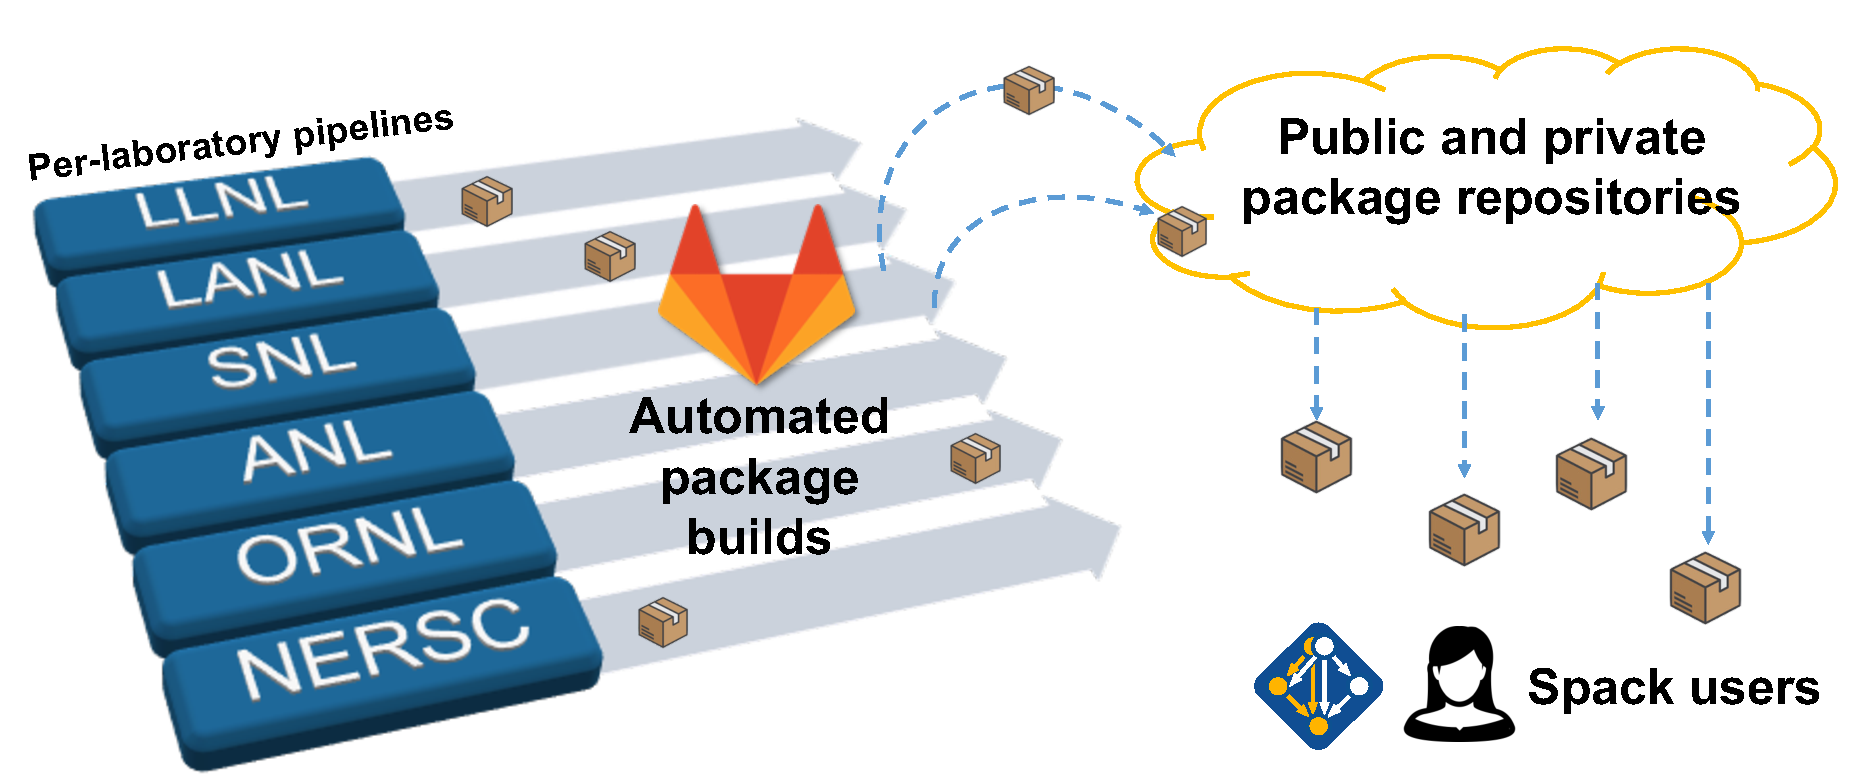
\includegraphics[width=.75\textwidth]{projects/2.3.6-NNSA/2.3.6.02-LLNL-ATDM/spack-pipelines.pdf}
\caption{Spack build pipelines at facilities will provide HPC-native binary builds for users.}
\end{figure}


\begin{itemize}
\item Spack won a 2019 R\&D 100 award as well as a Special Recognition
      as a Silver Medalist for being a ``Market Disruptor''.

\item Completed the implementation of {\it Spack Stacks}: an extension of Spack
      Environments that enable large combinatorial facility deployments to
      be specified in a single file.

\item Integrated Spack Environments and Spack Stacks with GitLab CI.  This
      allows hundreds of builds to be farmed out to runners at facilities and
      in the cloud.  Five organizations (NERSC, ANL, ORNL, NMC and the E4S team)
      were able to get pipelines working at their sites to automate builds.

\item Implemented a new prototype {\it concretizer} for Spack.  This version
      targets the NP-hard dependency resolution problem with an {\it
      Answer Set Programming} (ASP) based solver.  Preliminary results
      show that solves of complex Spack stacks can be completed in
      seconds and that this tool can handle complex backtracking cases
      and optimization of package criteria that the existing greedy
      concretizer cannot.

\item Spack has been selected as the package manager for Fugaku, Japan's
      flagship pre-exascale platform, and the team has been collaborating
      with RIKEN, Fujitsu, and SNL's Astra team to support the ARM
      platform.
\end{itemize}

\paragraph{Next Steps}
In FY20, the team will focus on:

\begin{itemize}
    \item Enhancing Spack's dependency model to treat compilers as
    dependencies, so that we can better model ABI compatibility in our
    stacks.

    \item Parallel builds for Spack: enable Spack to run inside a SLURM
    allocation to efficiently install a large number of packages at once.

    \item Better detection and integration with external dependencies.

    \item Continued support of LLNL ATDM, other labs' ATDM teams, and
          facilities.
\end{itemize}
